\documentclass[11pt]{article}
\usepackage[margin=1in]{geometry}
\usepackage[T1]{fontenc}
\usepackage{lmodern}
\usepackage{amsmath}
\usepackage{booktabs}
\usepackage{graphicx}
\usepackage{threeparttable}
\usepackage{tabularx}
\usepackage{setspace}
\usepackage[round,authoryear]{natbib}
\usepackage[hidelinks]{hyperref}
\usepackage{caption}
\captionsetup{font=small,labelfont=bf}
\graphicspath{{../outputs/step15/}{../outputs/step14/}{../outputs/step11/}}
\onehalfspacing
\newcolumntype{L}{>{\raggedright\arraybackslash}X}

\title{Frozen on the Last Open Version:\\ How Dependent Libraries Respond When an Open-Source Supplier Relicenses}
\author{Taejun Oh\thanks{Independent researcher. Email: \href{mailto:taejun.oh5@gmail.com}{\texttt{taejun.oh5@gmail.com}}.}}
\date{Working paper, November 2026}

\begin{document}
\maketitle

\begin{abstract}
\noindent Open-source software is code that anyone may use, modify and share. When the company behind an open-source library, a package of code that other programs build on, restricts the license of new versions, the projects built on that library must decide whether to follow. I study this decision after Akka, a widely used library for programs written in Java and Scala, moved to a restrictive license in 2022, using the build file each dependent project published with every release. At earlier launches about a quarter of dependents adopted the new version within eight months; under the new license, 4 percent did. Comparisons with libraries whose license did not change give a similar drop. Most projects stayed on the last open version, and when its security fixes ended, those that moved went mostly to a community fork, a copy of the last open version maintained by others. Why did they stay? When Elasticsearch, a widely used search engine, changed its license in 2021, the new terms bound only cloud companies that resold it, so ordinary projects built on it faced no new legal burden, and they kept upgrading. Akka projects that explained their choice mostly cited the new license, and those that said how it affected them pointed to clashes with their own open-source license, their foundation's rules or their users' needs. The evidence suggests that license restrictions travel down the chain of dependencies and can stall the ecosystem built on the supplier's code.

\medskip
\noindent\textbf{Keywords:} open source, software licensing, relicensing, forks, switching costs, hold-up, software supply chain\\
\noindent\textbf{JEL:} L17, L86, O34, D23
\end{abstract}

\newpage
\section{Introduction}

Open-source software is software whose source code, the human-readable instructions that make up a program, is published under a license that lets anyone use, modify and redistribute it. Much of it takes the form of libraries: packages of code that other programs incorporate instead of writing the same functions themselves. Open-source licenses work as a commitment. A permissive license lets anyone use, modify and redistribute the code with few conditions \citep{lerner2002,lerner2005}. A firm that releases a library under such a license therefore promises that users who build on it will not later be held up, that is, faced with new terms such as a fee or a restriction on use once they have already invested in building on the library. This promise persuades other developers to sink costs into the library, in the same way that second sourcing, a monopolist's licensing of a second producer, persuades buyers to adopt the monopolist's input \citep{farrell1988}. Since 2018 a series of single-vendor projects, open-source projects controlled by one company, have withdrawn that commitment for new versions: MongoDB, Elasticsearch, Redis, Terraform and Akka moved to licenses that restrict some commercial use, a change known as relicensing. Most of these moves were followed by a community fork: an independent copy of the last open version, which the open license allows anyone to make, maintained by volunteers or other companies: OpenSearch for Elasticsearch, Valkey for Redis, OpenTofu for Terraform and Pekko for Akka. Whether relicensing pays, for the vendor and for the ecosystem, depends on how the users who built on the code (its \emph{dependents}) respond. That response has not been measured systematically.

This paper measures that response for Akka, where each dependent's choice is on public record. Akka is a library, and many of its users are other open-source libraries and applications. When such a project publishes a release (a new version of its software) on Maven Central, the public repository through which libraries for the Java and Scala programming languages are distributed, it also publishes a build file that lists the libraries it needs and their versions. That file records, release by release, which Akka version the project chose. When Lightbend, the company that maintains Akka, relicensed it in September 2022, versions already released stayed under Apache 2.0, the permissive license Akka had used until then, and every dependent had to choose at each later release whether to stay on the last open version (\emph{freeze}), move to the restricted versions (\emph{upgrade}), move to the fork (\emph{switch}), publish both (\emph{dual}) or drop Akka (\emph{remove}). I build that record for every package that ever depended on Akka, from deps.dev, a public Google dataset of package metadata \citep{depsdev}, and follow each project from 2015 to late 2026.

\paragraph{The main finding.} Few dependents took the restricted versions. The clearest evidence compares launches of new Akka \emph{release series}, the sets of versions that share their first two numbers (2.6.0 to 2.6.21 form the 2.6 series). Figure~\ref{fig:outcomes} shows, for every project that was on the previous series at each launch, what it did in the following 240 days. At the three launches under Apache 2.0, in 2015, 2017 and 2019, between 20 and 27\% of projects moved to the new series. At the launch of 2.7, the first series under the Business Source License (BSL), which requires larger companies to buy a license to run the software in their live operations, 4\% did. Differences in the effort of upgrading cannot explain this, because 2.7 was the easier upgrade: Akka's migration guides say that 2.7 needs no configuration changes and removes no deprecated features or programming interfaces (APIs), while 2.6 removed some modules and dropped support for an older version of the Scala language, so some projects had to change their code to adopt it. Among 45 projects present at both launches, 22 adopted 2.6 but not 2.7, and none did the reverse. These comparisons use only Akka's own history, so they do not depend on how the users of any other library behaved.

\begin{figure}[t]
\centering
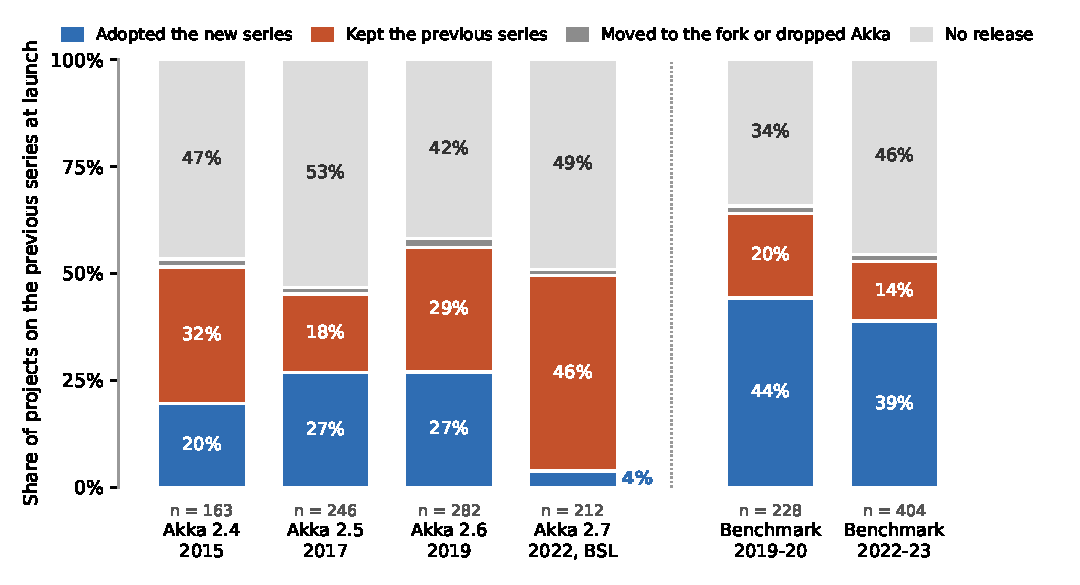
\includegraphics[width=0.92\textwidth]{fig_outcomes.pdf}
\caption{Where projects went within 240 days of each launch. All projects on the previous series at the launch, including those that published no release. ``Kept the previous series'': released, and at least one release still declared the previous series. Benchmark: dependents of cats-core and jackson-module-scala, for launches in 2019--20 and 2022--23.}
\label{fig:outcomes}
\end{figure}

The size of the drop is 30 percentage points against the 2019 launch (95\% confidence interval 19 to 41). This estimate reweights the 2019 projects to resemble the 2022 projects in size, age and the Akka modules they use; without reweighting the drop is 23 points. Adoption did not trend across the earlier launches (27\% in both 2017 and 2019), so allowing for a trend changes little: the drop is 28 points after subtracting the change from 2017 to 2019, and 35 points measured against a straight-line trend through all three Apache launches. Libraries whose license did not change give a similar answer. Comparing Akka's change between its 2019 and 2022 launches with the change for two widely used Scala libraries that do not compete with Akka gives a drop of 25 points.

Most projects that did not adopt stayed on the last open version. Among projects that kept releasing, 97 of the 100 that did not adopt 2.7 still used 2.6 in their releases. Across all projects, the share that stayed on the old series was 14 to 25 points higher after the 2022 launch than after the 2019 launch, depending on the horizon and the weighting, and moves to the fork within the year were rare. The share of projects that published no release also rose, by up to 15 points. This rise depends on the weighting and partly reflects projects releasing later in the year. When security fixes for the open series ended in September 2023, frozen projects that moved went mostly to the fork: of 129 projects frozen in June 2023, 39 had moved to Pekko by June 2024 and 5 had upgraded, about eight to one. A second estimate, from quarterly panel data, points the same way. It relies on the assumption that Akka projects and a comparison group would have followed parallel trends without the license change, and it does not survive small departures from that assumption, so I report it as fragile.

\paragraph{Why dependents stayed.} Section~\ref{sec:model} sets out two reasons a dependent might refuse the new versions and one reason it might take them anyway. The first reason to refuse is the \emph{legal cost}: the burden the new license places, now, on the project and on its users. The second is \emph{hold-up}: the fear that a supplier that has changed its terms once will change them again. The reason to take the new versions anyway is \emph{dependency-graph availability}. A project often uses Akka both directly and through other Akka-based libraries, such as a web-server component or a database connector. It can move to the fork cleanly only once each of those libraries has also been released for the fork; such a release is called a \emph{port}. Until then, leaving Akka means porting, replacing or dropping those libraries itself. A project whose libraries lack ports may therefore stay with Akka, and take the restricted versions once the open versions stop receiving fixes. Each channel predicts a different pattern. Elasticsearch, a widely used search engine, is the main contrast. It was relicensed in 2021 under a license that restricts only companies that sell access to it as a cloud service, so its dependents faced almost no legal cost; but they had as much reason as Akka's dependents to distrust a supplier that had changed its terms. They kept upgrading. After the change, Elasticsearch dependents moved into restricted versions in 35\% of the quarters in which they released; Akka dependents did so in 6\%. In their issue trackers, the public lists of bug reports and change requests that projects keep on GitHub, the main website for hosting open-source code, most Akka dependents that state a motive give the license as the reason. The mechanism they describe is more often a license-compatibility rule than a fee. A language model coded these motives, and the author's own coding of a sample of 60 repositories, done without seeing the model's codes, agrees closely. Three tests of hold-up, in Section~\ref{sec:channels}, find no support for it. A direct test of the legal cost uses each project's number of downstream users, the other packages that depend on it; it finds no effect and has little power. The license-compatibility explanation is therefore suggestive.

\paragraph{Contribution.} The paper contributes to three literatures. First, to the economics of open-source licensing and commitment \citep{lerner2002,lerner2005,farrell1988,august2021,casadesus2006,casadesus2011}, which explains why firms choose open or restrictive licenses and models the consequences. To my knowledge this is the first systematic measurement of downstream version adoption after a relicensing, covering the full population of dependents with comparison groups. Second, to empirical work on relicensing, which has studied the organizations contributing to relicensed projects and to their forks \citep{foster2024}, cloud providers' contributions around the Redis license change \citep{han2026}, community responses and hard forks \citep{foster2026}, the incidence of license events \citep{dmitrenko2026} and project activity after a change from a restrictive to a permissive license \citep{jahanshahi2026}, but not the dependents. Earlier work on the users' side measured interest in projects at one point in time \citep{stewart2006}, or compared periods before and after license changes, mostly from one open license to another, without a comparison group \citep{santos2017}. Third, to software-engineering work on dependency updating and library migration \citep{kula2018,he2021,miller2025}, which documents that projects often keep outdated or abandoned dependencies and studies when they migrate between libraries. This paper separates the freezing caused by one dated event, a relicensing, from that background. The coded dataset of dependents' choices is released with the paper.

Section~\ref{sec:setting} describes the two events. Section~\ref{sec:model} sets out the model and the three channels. Section~\ref{sec:data} explains the data. Section~\ref{sec:launch} presents the launch evidence, Section~\ref{sec:panel} the panel and the period after patches ended, and Section~\ref{sec:channels} the evidence on channels. Section~\ref{sec:threats} collects the threats to validity, and Section~\ref{sec:discussion} discusses implications.

\section{Setting}\label{sec:setting}

\paragraph{Akka and its license change.} Akka is a toolkit for concurrent and distributed software, that is, software that performs many tasks at the same time, often across several machines. It runs on the Java Virtual Machine (JVM), the runtime on which Java and Scala programs run. It is written in Scala and maintained by Lightbend. It is used directly by applications and indirectly through frameworks and libraries such as the Play web framework, the stream-processing system Apache Flink and many connectors to databases and message queues. On 7 September 2022 Lightbend announced that new versions would be released under the Business Source License 1.1, a source-available license: anyone may read and modify the code, but production use, that is, running it in a company's live operations, needs a commercial license. The first stable BSL releases of every module (the separately released parts of the toolkit) followed on 19--21 October 2022. Each BSL version reverts to Apache 2.0 three years after its release. From version 2.9 (October 2023) Akka was published only in Lightbend's own repository, which requires an account token, and from October 2024 new versions also required a license key.

In 2022 the commercial license was free for companies with revenue below US\$25 million. Above that threshold the price list, billed annually, was US\$1,995 per core per year (Standard) or US\$2,995 (Enterprise, minimum 40 cores). A \emph{core} here is a processor core on the servers that run the software in production; the price list defined it as ``a hardware core / vCore / vCPU'', so a cloud virtual CPU counts as one core. The fee therefore scales with the computing capacity that runs Akka. Revenue decides only whether a company pays at all. A deployment on 100 virtual CPUs at Standard pricing would cost about US\$200,000 a year. Production systems are sized for peak load and redundancy, so the count of licensable cores can be well above what average traffic requires. Non-production use was free.

A library that depends on Akka does not itself pay. But Lightbend's published answers to frequently asked questions (FAQ) stated that code mixing BSL and open components ``will still require a commercial license for production usage of the BSL licensed code''. A library that moves to a BSL version therefore passes the license requirement on to every company that runs software built on it. For the open-source dependents studied here, this passed-on requirement is the constraint that matters.

Released versions stayed under Apache 2.0. Lightbend's initial FAQ promised no further updates to them; within days it added that critical security fixes (\emph{patches}) for the 2.6 series would continue until September 2023. The last Apache patch, 2.6.21, was released on 21 June 2023. The community fork, Apache Pekko, is based on Akka 2.6.20. It released its core modules on 10 July 2023 and the remaining modules between July and October 2023. Pekko cannot copy code released under the BSL, so it could not take the features added to Akka after 2.6 until the versions that added them converted to Apache 2.0, three years after their release.

\paragraph{Elasticsearch.} On 14 January 2021 Elastic announced that new versions of Elasticsearch would be released under a choice of two licenses, the Elastic License 2.0 (ELv2) and the Server Side Public License (SSPL). Version 7.10.2 was the last Apache release; 7.11.0, released on 10 February 2021, was the first restricted one. Apart from a ban on circumventing license keys, ELv2 restricts only parties that provide the software to others as a hosted or managed service. Amazon Web Services (AWS), Amazon's cloud business, forked the code as OpenSearch, which reached version 1.0 in July 2021. For library dependents the relevant artifacts (published packages) are the server and the high-level REST client, the library through which Java programs send requests to an Elasticsearch server. Both were relicensed. Elastic later introduced a new Apache-licensed Java client (September 2021), deprecated the old client and dropped it in 8.0, and from 7.14 its clients refused to connect to non-Elastic servers. In August 2024 Elastic added the AGPL, an approved open-source license, as a third option.

The paper uses the main difference between the two events: whom the license restricts. Akka's BSL reaches every company that runs Akka-based software in production, through any library in between. ELv2 reaches only hosting providers, so an ordinary library that depends on Elasticsearch, and that library's users, face no new legal constraint.

\section{A model of the dependent's choice}\label{sec:model}

A supplier relicenses all new versions at date $\tau$; versions released before $\tau$ stay open. A dependent $i$, usually itself a library, chooses at each release $t>\tau$ among freezing on the last open series (F), upgrading to a restricted version (U), switching to the fork (S), dual publishing (D) and removing the dependency (R). With $v$ the value of the supplier's functionality, the payoffs are
\begin{align*}
V_F &= v - d(t), \\
V_U &= v + g(t) - a_i - e_i(\rho)\,c - h\,\Delta\pi_i, \\
V_S &= v + q(t) - k_i(t),
\end{align*}
and $V_D = \max(V_U,V_S) + \varepsilon_D - m$. Here $d(t)$ is the cost of staying on an ageing version, which jumps when patches for the open series end; $g(t)$ is the value of the improvements in restricted versions; $a_i$ is the one-time cost of changing the project's code to the new series; and $q(t)$ is the fork's quality. Dual publishing means releasing two builds of the project, one on Akka and one on the fork. It keeps the better of the two options, plus a gain $\varepsilon_D$ from serving users of both, at a maintenance cost $m$. Each option also carries a random term, independent across projects and options, for reasons the model leaves out. The remaining three terms are the three channels. $e_i(\rho)\,c$ is the legal cost. In the hold-up term $h\,\Delta\pi_i$, $\Delta\pi_i$ is the dependent's revision of belief: the increase, caused by the relicensing, in the probability it assigns to the supplier restricting the terms further; $h$ is the loss it would suffer if that happened. $k_i(t)$ is the cost of switching to the fork. Each is defined below.

\paragraph{Legal cost, $e_i(\rho)\,c$.} This is the present, known burden of the license. $c$ is the cost of compliance per exposed unit: a fee, registration, legal review, or a conflict with a license rule the project must obey. $e_i(\rho)$ is the exposure of $i$'s user base to a license with restriction scope $\rho$, which describes the kinds of user the license restricts. If $i$'s users fall into classes $j$ with shares $s_{ij}$ and the license restricts the set $R(\rho)$, then $e_i(\rho)=\sum_{j\in R(\rho)} s_{ij}$. Under Akka's BSL, $R$ contains every commercial production user, so $e_i$ is positive and often large; under ELv2, $R$ contains only hosting providers, so $e_i\approx 0$ for a typical library. For the fee part of $c$, exposure has two dimensions: whether a user is above the revenue threshold, and how many cores it runs. For the open-source libraries observed here the legal cost is the passed-on requirement described in Section~\ref{sec:setting}, and a project's own license or its foundation's policy may also forbid a BSL dependency outright.

\paragraph{Hold-up, $h\,\Delta\pi_i$.} Hold-up arises when one party, after the other has made investments that are costly to reverse, changes the terms in its own favor \citep{klein1978,williamson1985}. Here the investment is the dependent's code and design built around Akka, and the team's knowledge of it; the change of terms is the relicensing. A relicensing shows that the supplier is willing to change terms, so the dependent raises the probability it assigns to further restriction, such as higher prices, tighter terms or a license-key requirement. $\Delta\pi_i$ is the size of that increase, and $h$ is the loss if the supplier does restrict further. An open license is a commitment device against hold-up \citep{lerner2002}: because everyone keeps the right to use and modify the released code, the supplier cannot later change the terms on it. Withdrawing that commitment affects every user, including those that face no cost under the current terms, so hold-up, unlike the legal cost, arises under either license.

\paragraph{Dependency-graph availability, $k_i(t)$.} This channel works in the other direction: it can keep a dependent on the supplier's versions. To switch cleanly to the fork, a project needs a port of every Akka-based library it uses. The switching cost is
\[
k_i(t)=k_0+b\cdot(\text{number of Akka-based libraries $i$ uses that have no fork version at $t$}),
\]
where $k_0$ is the cost of the switch itself and $b$ is the extra cost for each library the project must port, replace or drop on its own. The cost falls when the last port a project needs arrives. Before the fork's first release on 10 July 2023, switching was impossible: $k_i(t)=\infty$ for every project. Between the fork's core release and the last port a project needs, switching is possible but costly. While $k_i$ is high, a project that finds the open series too old (when $d(t)$ jumps) chooses mainly between upgrading and staying frozen, so missing ports raise the chance that it takes the restricted versions. No fork existed during any of the launch windows studied in Section~\ref{sec:launch}, including that of 2.7, so this channel was the same at every launch and cannot explain the fall in adoption there. It matters after mid-2023. This channel is sometimes called coordination. It is narrower than strategic coordination among dependents, in which a project's value of switching depends on whether its peers and users also switch \citep{farrell1985,farrell2007}. The paper measures only whether the ports a project needs exist, and does not test peer coordination.

\begin{table}[t]
\centering
\begin{threeparttable}
\caption{Three channels and what each predicts}\label{tab:channels}
\footnotesize
\begin{tabularx}{\textwidth}{p{3.2cm}LLL}
\toprule
& Legal cost & Hold-up & Dependency-graph availability \\
\midrule
Model term & $e_i(\rho)\,c$ & $h\,\Delta\pi_i$ & $k_i(t)$ \\
What it is & Present burden of the license on the project and its users & Fear that the supplier will change the terms again, after the project has invested in its code & Whether every Akka-based library the project uses has a fork version (a port) \\
Effect on taking restricted versions & Lowers it & Lowers it & Raises it while ports are missing, since leaving is costly \\
Who stops upgrading & Projects whose users are restricted & Also projects with no restricted users & Not a reason to stop \\
BSL against ELv2 & Freeze under BSL, not under ELv2 & Similar response under both & No prediction \\
When restricted versions become open (BSL conversion) & Projects take the converted versions & Projects stay away & No prediction \\
Supplier's other, unrelicensed libraries & Use unchanged & Use falls & No prediction \\
Timing of switching & At the event, or when fees bind & At the event & When the last required port arrives \\
\bottomrule
\end{tabularx}
\end{threeparttable}
\end{table}

Table~\ref{tab:channels} summarizes what each channel predicts. A dependent that stays with the supplier chooses between upgrading and freezing, and its probability of upgrading increases with the gain from upgrading,
\[
V_U - V_F = g(t) + d(t) - a_i - e_i(\rho)\,c - h\,\Delta\pi_i .
\]
This gives the predictions the paper takes to the data. (P1) Under the BSL, upgrading falls relative to the supplier's own earlier launches and to libraries without relicensing. (P2) Under ELv2 the legal term is near zero, so upgrading falls only through hold-up. (P3) Comparing the two events therefore isolates the legal term, provided that dependents of both suppliers revised their beliefs about further restriction by similar amounts and that the other terms are similar; with only two events this cannot be tested. (P4) The fall in upgrading consists of fewer moves into restricted versions. Raises within the open series fall only because no new open versions are released. (P5) When patches for the open series end, $d(t)$ jumps and frozen dependents leave F: toward S if the legal term is large, toward U if it is small or if the ports they need are missing. (P6) Given that the fork exists, switching rises when the last port a dependent needs becomes available, and until then projects missing a port upgrade more often. (P7) A large migration cost $a_i$ suppresses upgrading regardless of license; this applies to Elasticsearch's client change.

\section{Data and measurement}\label{sec:data}

\subsection{Where the data come from}

\paragraph{Maven Central and build files.} Maven Central is the main public repository of Java and Scala libraries, run by Sonatype. Every published package is identified by three coordinates, written \texttt{group:artifact:version}; Akka's core module, for instance, has group \texttt{com.typesafe.akka}, artifact \texttt{akka-actor\_2.13} and version \texttt{2.6.20}. The suffix \texttt{\_2.13} is a Scala convention: Scala versions are not binary compatible (code compiled for one Scala version cannot be combined with libraries compiled for another), so each module is published separately for Scala 2.12, 2.13 and 3, and one project often publishes several artifacts, one per Scala version, that reflect a single choice of Akka version. A published version can never be changed or deleted, so a release history on Maven Central is a reliable record of what a project shipped and when.

With every release a project publishes a POM (Project Object Model), a short XML file that describes the package. It names the package, its license, its source repository, and the libraries it needs with their versions. Figure~\ref{fig:pom} shows a simplified example. Build tools such as Maven, Gradle and sbt read POMs to decide which libraries to download, and projects built with sbt or Gradle publish POMs generated from their build files. A POM therefore records the Akka version a project chose for each release. I call this the \emph{declared} version: the version listed in the build file the project published.

\begin{figure}[t]
\centering
\begin{minipage}{0.86\textwidth}
\footnotesize
\begin{verbatim}
<project>
  <groupId>io.example</groupId>
  <artifactId>example-streams_2.13</artifactId>
  <version>1.4.0</version>
  <licenses><license><name>Apache-2.0</name></license></licenses>
  <scm><url>https://github.com/example/example-streams</url></scm>
  <dependencies>
    <dependency>                              <!-- coded as: on the open series -->
      <groupId>com.typesafe.akka</groupId>
      <artifactId>akka-actor_2.13</artifactId>
      <version>2.6.20</version>
    </dependency>
    <dependency>                              <!-- test only: ignored -->
      <groupId>org.scalatest</groupId>
      <artifactId>scalatest_2.13</artifactId>
      <version>3.2.15</version>
      <scope>test</scope>
    </dependency>
  </dependencies>
</project>
\end{verbatim}
\end{minipage}
\caption{A simplified POM (build file) for a hypothetical library that depends on Akka. The release would be coded as on the open series (2.6). Had it listed \texttt{akka-actor\_2.13:2.8.5}, it would be coded as on restricted versions; had it listed \texttt{org.apache.pekko:pekko-actor\_2.13:1.0.2} only, as on the fork.}
\label{fig:pom}
\end{figure}

\paragraph{deps.dev and BigQuery.} deps.dev (Open Source Insights) is a Google project that reads the package registries, including Maven Central, collects each package version's metadata (publication date, license, source-repository link and the full content of its POM), and computes dependency graphs. It publishes periodic snapshots of these data as public tables in BigQuery, Google's database service for large analytical queries. A query reads the stored snapshot; it does not contact Maven Central. I use the snapshot of 2 November 2026: \texttt{MavenRequirements}, which holds the declared content of every POM (dependencies, dependency management, properties and parent), and \texttt{PackageVersions}, which holds publication dates, licenses and source-repository links. I extract every version of every package that ever declared an Akka, Pekko or Play dependency (7,574 packages and 445,321 declarations of these three libraries, called \emph{Akka-family} declarations below), and the same for the dependents of the comparison libraries. The extracts are cached, so the analysis re-runs offline from the replication package.

\subsection{Coding a release}

\paragraph{Declared and resolved versions.} The coding uses declared versions. The alternative is the resolved version: the one a build tool finally downloads after settling conflicting requirements among all the libraries in a build. Declared versions keep upgrades to Akka 2.9 and later visible. Those versions are not on Maven Central, so deps.dev cannot resolve them, but a dependent that publishes to Maven Central still lists them in its own POM (15 projects in the Akka risk set, defined below, do).

\paragraph{Where POMs get complicated.} In several cases the version in a POM is not written out as a plain number, and the coding has to work it out.
\begin{itemize}\itemsep1pt
\item \emph{Properties and parent POMs.} A version is often a variable (\texttt{\$\{akka.version\}}) defined in the same file or in a parent POM it inherits from. Variables are substituted, and parent POMs were fetched from Maven Central where needed.
\item \emph{Dependency management and bills of materials.} A POM can fix the versions of many libraries in one section (dependency management). A project can list \texttt{akka-actor} without a version and import a separate POM that fixes versions for a family of libraries. Of the 445,321 Akka-family declarations, 94.1\% carry a literal version, 4.0\% are resolved through dependency management or an imported bill of materials, and 1.9\% cannot be resolved.
\item \emph{Scopes.} Test-scope and optional dependencies are ignored. A \texttt{provided} dependency is needed to compile but supplied by the user at run time, so the user chooses the version; such projects are kept but flagged.
\item \emph{Shading.} A project can copy a library's code into its own package and drop the dependency from its POM. Apache Flink did this with Akka, and was recoded by hand.
\end{itemize}

\paragraph{Validation.} For a sample drawn separately from each outcome group, the coding was compared with the build files in the projects' own repositories. Raw agreement was 94.7\% and Cohen's $\kappa$ was 0.93; $\kappa$ measures agreement after removing the agreement expected by chance, so that 1 is perfect agreement and 0 is chance. The comparison led to three corrections: for projects that copy Akka's code into their own (shading, above), for a third-party library that wraps Akka, and for repositories that had moved.

\paragraph{Units.} A project is a GitHub repository, taken from the package's source-repository link and normalized; packages without a link are grouped by Maven group ID. Each release of each artifact is coded by the Akka versions it declares: on the open series, on restricted versions, on the fork, mixed, or none. Vendor-affiliated projects (owners \texttt{lightbend}, \texttt{akka}, \texttt{playframework}) are excluded from all estimates. The Akka \emph{risk set}, used in the panel design, consists of the projects that had at least one release between 7 September 2020 and 6 September 2022 and whose latest release of at least one artifact before the event declares a non-test, non-optional Akka dependency.

\begin{table}[t]
\centering
\begin{threeparttable}
\caption{Terms used in the paper}\label{tab:terms}
\footnotesize
\begin{tabularx}{\textwidth}{p{3.4cm}L}
\toprule
Term & Meaning \\
\midrule
Declared version & The Akka version listed in the build file (POM) a project published with a release \\
Release series & All versions sharing the first two numbers, e.g.\ 2.6.0 to 2.6.21 \\
Launch & The first stable release of a new series (2.6.0 on 6 Nov 2019; 2.7.0 on 19 Oct 2022) \\
Active & Published at least one release of any of its packages in the window \\
Adopt (launch design) & Declares a stable version of the new series or later in a release within the window \\
Freeze & Keeps declaring the previous, open series, and no restricted version \\
Upgrade (panel, M1) & Any raise of the declared version, including patches within 2.6; a \emph{raise into restricted versions} is the part that moves to BSL versions \\
Switch & Declares only the fork (Pekko) \\
Dual & Maintains artifacts on both Akka and the fork \\
Remove & Declares no Akka version of any kind and no fork version. A project that still declares the open series is coded as freeze \\
Port & A version of an Akka-based library built on the fork \\
\bottomrule
\end{tabularx}
\end{threeparttable}
\end{table}

\paragraph{Terms.} Table~\ref{tab:terms} lists the terms used in the rest of the paper.

\paragraph{What the data cannot see.} Three limits follow from the source. First, only projects that publish to Maven Central are observed. Closed-source applications and internal services, which are the parties the BSL actually charges, never publish there. Second, a project that moved its own publishing off Maven Central, for example to Lightbend's repository when it adopted 2.9, would look inactive or frozen after the move. Third, 1.9\% of declarations cannot be resolved; if these were concentrated among projects that took BSL versions, the paper would understate upgrades.

\paragraph{Comparison groups.} For the launch design, two benchmarks are used. The first consists of dependents of cats-effect and fs2, two libraries from Typelevel, an open-source organization whose libraries are an alternative to Akka for concurrent programming in Scala. These two libraries compete with Akka for the same developers, so Akka's license change may also have affected their adoption. The second benchmark avoids this problem. It consists of libraries chosen by a rule: Scala libraries that do not offer concurrency (including effect systems), streaming or HTTP functions, that launched a new series within six months of both Akka launches, and that had at least 30 active dependents at each launch. Two libraries qualify: cats-core, a general functional-programming library, and jackson-module-scala, a JSON serialization library. For the panel design, the comparison group for Akka consists of projects that declare cats-effect, ZIO, fs2 or http4s and no Akka; for Elasticsearch it consists of dependents of Apache SolrJ, Lucene core and the HBase client, libraries for other search and database systems.

\section{Launch evidence: who adopted the new series?}\label{sec:launch}

\subsection{Design}

\paragraph{Cohorts.} Each Akka launch defines a cohort, the group of projects that were using the previous series when the launch happened: 2.4.0 (30 September 2015), 2.5.0 (12 April 2017) and 2.6.0 (6 November 2019) under Apache 2.0, and 2.7.0 (19 October 2022) under the BSL. A project enters the cohort of a launch at date $L$ if it released at least once in $[L-365, L)$ and if, for at least one of its artifacts, the latest release before $L$ declares a non-test, non-optional dependency on the previous series, and the new series is published for that artifact's Scala version. Projects already on the new series or its milestones (test versions published before the launch), vendor-owned projects and projects that also declare Play are excluded, since Play, not the project, sets their Akka version. Membership depends only on releases before the launch.

\paragraph{Outcomes.} Within $H=240$ days of the launch each project falls in exactly one of four classes: it \emph{adopted} the new series; it \emph{kept the previous series} (it released, and some release still declared the previous series); it \emph{left} (it released, but only with the fork or with no Akka); or it published \emph{no release}. The horizon is set by the calendar: it ends each cohort's window before the first event that would push projects to reconsider their Akka version for other reasons (for 2.7, the end of 2.6 patches and the arrival of Pekko in mid-2023).

\paragraph{Estimands.} The main estimate is the within-Akka contrast: the share of the 2.7 cohort that adopted within 240 days minus the same share for the 2.6 cohort, with projects that published no release counted as non-adopters. The 2.5 and 2.4 launches measure the trend across launches. The \emph{trend-adjusted contrast} subtracts the change from 2.5 to 2.6; a second version subtracts a linear trend through 2.4, 2.5 and 2.6. The earlier cohorts are reweighted so that their characteristics before the launch match those of the 2.7 cohort. The weights are odds weights from a logit model of membership in the 2.7 cohort, with predicted probabilities trimmed to $[0.05,0.95]$ to avoid extreme weights. The characteristics are the number of releases and artifacts, any Scala 2.13 artifact, project age, days since the last change of declared Akka version, and whether the project uses the cluster, persistence or HTTP modules. Standard errors are clustered by GitHub owner, which allows the outcomes of projects with the same owner to be correlated. The $p$-values come from a restricted wild cluster bootstrap with Rademacher weights \citep{cameron2008}, a resampling method that stays accurate when clusters are few or uneven in size.

The benchmark comparison is a difference-in-differences: it compares the change in adoption between the early and late launches for Akka with the same change for the benchmark libraries. It is estimated on data with one row per project and cohort,
\[
Y_{ic} = \alpha + \beta\,\text{Akka}_c + \gamma\,\text{Late}_c + \theta\,(\text{Akka}_c\times \text{Late}_c) + \varepsilon_{ic},
\]
where Akka marks the Akka cohorts, Late marks the 2022--23 launches, and $\theta$ is the estimate; each group's early cohort is reweighted to its late cohort. The comparison assumes that, without the license change, adoption at launch would have changed for Akka as it did for the benchmark. This needs to hold only for one outcome at two points in time, which is less demanding than parallel trends over many quarters.

\paragraph{What else changed at the 2.7 launch.} The supplier changed two things at once: the license, and the release pattern that followed (2.7.0 received no patch before 2.8.0 in March 2023, and 2.6 received no patch inside the window). The estimates measure the two together. Two other differences between the 2.6 and 2.7 launches should have made 2.7 easier to adopt, so they work against finding a fall. Akka's migration guide for 2.6 lists dropped Scala 2.11 support, removed modules and a new default networking layer, while the guide for 2.7 says that ``no configuration changes are needed''. And during the 2.6 window the previous series still received patches, while during the 2.7 window it received none.

\paragraph{Order of the analyses.} I designed the launch comparison after the panel estimate (Section~\ref{sec:panel}) had proved fragile. By then the panel data had already shown that few projects took 2.7, so the result for the 2.7 launch was partly known, and the adoption shares among active projects were known before the estimates in Tables~\ref{tab:akka} and~\ref{tab:bench} were computed. The results for the 2.6, 2.5 and 2.4 launches and for the benchmarks were computed afterward.

\subsection{Results}


\paragraph{Across Akka launches.} Figure~\ref{fig:outcomes} shows the four outcomes at each launch. Besides the fall in adoption from 20--27\% to 4\%, the share that kept the previous series rose to 46\%, against 18 to 32\% at the earlier launches. Moves to the fork or away from Akka were below 2.5\% in every cohort; no fork existed in any of the windows. The benchmark's adoption share fell only slightly, from 44 to 39\%.

\begin{table}[t]
\centering
\begin{threeparttable}
\caption{Within-Akka launch contrasts: adoption within 240 days}\label{tab:akka}
\footnotesize
\setlength{\tabcolsep}{4pt}
\begin{tabularx}{\textwidth}{Lcc}
\toprule
& Weighted & Unweighted \\
\midrule
\multicolumn{3}{l}{\emph{All projects in the cohort (inactive counted as non-adopters)}} \\
2.7 minus 2.6 (main estimate) & $-0.302$ $[-0.41,-0.19]$, $p<0.001$ & $-0.232$ $[-0.29,-0.17]$ \\
2.6 minus 2.5 (placebo, both Apache) & $-0.025$ $[-0.16,0.11]$, $p=0.72$ & $+0.001$ $[-0.08,0.08]$ \\
Trend-adjusted: (2.7 $-$ 2.6) minus (2.6 $-$ 2.5) & $-0.278$ $[-0.49,-0.07]$, $p=0.014$ & $-0.233$ $[-0.35,-0.11]$ \\
2.7 against linear trend through 2.4, 2.5, 2.6 & $-0.353$ $[-0.55,-0.15]$ & $-0.281$ $[-0.39,-0.18]$ \\
2.7 minus 2.6, 365-day horizon & $-0.356$ $[-0.47,-0.24]$ & $-0.264$ $[-0.33,-0.20]$ \\
\midrule
\multicolumn{3}{l}{\emph{Projects active within 240 days}} \\
2.7 minus 2.6 & $-0.402$ $[-0.54,-0.26]$ & $-0.389$ $[-0.48,-0.30]$ \\
2.6 minus 2.5 & $-0.190$ $[-0.36,-0.02]$ & $-0.111$ $[-0.24,0.02]$ \\
Trend-adjusted & $-0.211$ $[-0.48,0.06]$, $p=0.14$ & $-0.279$ $[-0.46,-0.09]$ \\
Lee bounds on 2.7 minus 2.6, always-active projects & \multicolumn{2}{c}{$[-0.454,-0.315]$; 95\% CI $[-0.62,-0.16]$} \\
\midrule
\multicolumn{3}{l}{\emph{Within project: 45 projects active at both launches}} \\
Adopted 2.6 only / 2.7 only / both / neither & \multicolumn{2}{c}{22 / 0 / 2 / 21; exact McNemar $p<0.001$} \\
\bottomrule
\end{tabularx}
\begin{tablenotes}\footnotesize
\item Cohorts: 2.4 (163 projects), 2.5 (246), 2.6 (282), 2.7 (212). Linear probability models; brackets are 95\% confidence intervals with owner-clustered standard errors; $p$-values from a restricted wild cluster bootstrap (9,999 draws). Weighted rows reweight earlier cohorts to the 2.7 cohort's pre-launch covariates; after weighting, all standardized differences between 2.6 and 2.7 are within 0.26. The bootstrap CI of the Lee bounds clusters by owner.
\end{tablenotes}
\end{threeparttable}
\end{table}

Table~\ref{tab:akka} gives the estimates summarized in the introduction. The placebo, the same comparison between the two Apache launches 2.5 and 2.6, is close to zero, which is why adjusting for the trend across launches barely changes the main estimate. At 365 days the drop is larger. The reweighting balances 2.6 against 2.7 well, but it cannot balance the 2015 and 2017 cohorts against 2022, because Scala 2.13 builds did not exist before 2019; for the trend-adjusted rows the unweighted estimates are therefore the more reliable.

Counting only projects that kept releasing gives a larger contrast, $-0.40$. But this measure also shows a fall between the two Apache launches ($-0.19$ weighted), where no license changed, because the share of active projects rose from 47\% in the 2017 cohort to 58\% in the 2019 cohort, which changed who counts as active. For this reason the main estimate counts all projects. Because the license may itself have changed which projects kept releasing, Table~\ref{tab:akka} also reports Lee bounds \citep{lee2009}. They drop the highest- or the lowest-adopting active projects from the cohort with the higher activity share until both cohorts have the same share, and so bound the effect for projects that would have released under either license. Even in the least favourable case the fall exceeds 31 points.

Comparing the same projects across launches addresses the concern that the 2022 cohort simply consisted of different projects. Forty-five projects were active on the previous series at both launches. Twenty-two adopted 2.6 but not 2.7, none adopted 2.7 but not 2.6, two adopted both and 21 neither (exact McNemar test for paired outcomes, $p<0.001$).

\begin{table}[t]
\centering
\begin{threeparttable}
\caption{Difference-in-differences against benchmark libraries}\label{tab:bench}
\footnotesize
\setlength{\tabcolsep}{3pt}
\begin{tabularx}{\textwidth}{Lccc}
\toprule
& \multicolumn{2}{c}{All projects} & Active projects \\
\cmidrule(lr){2-3}\cmidrule(lr){4-4}
Benchmark & Weighted & Unweighted & Weighted \\
\midrule
Non-competing, pooled & $-0.245$ $[-0.41,-0.08]$, $p=0.006$ & $-0.177$ $[-0.31,-0.05]$ & $-0.424$ $[-0.60,-0.25]$ \\
\quad cats-core & $-0.177$ $[-0.35,-0.00]$, $p=0.06$ & $-0.128$ $[-0.27,0.01]$ & $-0.415$ $[-0.60,-0.23]$ \\
\quad jackson-module-scala & $-0.224$ $[-0.47,0.03]$, $p=0.10$ & $-0.315$ $[-0.50,-0.13]$ & $-0.214$ $[-0.50,0.07]$ \\
Typelevel (cats-effect, fs2) & $-0.178$ $[-0.36,0.00]$, $p=0.06$ & $-0.035$ $[-0.15,0.08]$ & $-0.408$ $[-0.60,-0.22]$ \\
Pooled with Typelevel & $-0.181$ $[-0.32,-0.04]$, $p=0.01$ & $-0.104$ $[-0.20,-0.01]$ & $-0.375$ $[-0.55,-0.20]$ \\
\midrule
\multicolumn{4}{l}{\emph{Benchmark shares, 2019--20 / 2022--23}} \\
Non-competing: active; adopted & \multicolumn{3}{c}{0.66 / 0.54; \quad 0.44 / 0.39} \\
Typelevel: active; adopted & \multicolumn{3}{c}{0.76 / 0.57; \quad 0.67 / 0.48} \\
Lee bounds, active, against Typelevel & \multicolumn{3}{c}{$[-0.443,-0.146]$; 95\% CI $[-0.64,0.02]$} \\
\bottomrule
\end{tabularx}
\begin{tablenotes}\footnotesize
\item Difference-in-differences of adoption within 240 days, Akka 2.6/2.7 against each benchmark's launches in 2019--20 and 2022--23. Non-competing benchmarks are chosen by the rule in Section~\ref{sec:data}: of 931 Scala libraries with a new series in both windows, the 20 with the most dependents were extracted and two had at least 30 active dependents at both launches (cats-core 2.1.0 and 2.8.0; jackson-module-scala 2.10.0 and 2.14.0). A project in several benchmarks of one period is counted once. Brackets and $p$-values as in Table~\ref{tab:akka}.
\end{tablenotes}
\end{threeparttable}
\end{table}

\paragraph{Against benchmark libraries.} Table~\ref{tab:bench} compares Akka with the benchmarks. Among active projects, every benchmark gives a drop of about 40 points except the small jackson-module-scala group. On all projects, the pooled non-competing benchmark gives $-0.25$ ($-0.18$ unweighted). The Typelevel benchmark alone gives a smaller and imprecise estimate, because activity among Typelevel dependents fell from 76 to 57\% between its two launches, which lowered its adoption share among all projects. This fall in activity is not limited to the cohorts. Among all projects in the comparison data, the share that released in a year, out of those that had released the year before, fell from 0.67 in 2020 to 0.59 in 2022; among Akka-dependent projects it stayed near 0.61. Jackson-module-scala, the one benchmark whose activity did not fall (59\% in both windows), gives $-0.32$ unweighted. Two limits remain: only two libraries met the size rule, and the pooled estimate is driven mostly by cats-core, which belongs to the same Typelevel family as the first benchmark; jackson-module-scala, the only benchmark outside that family, is small.

\begin{figure}[t]
\centering
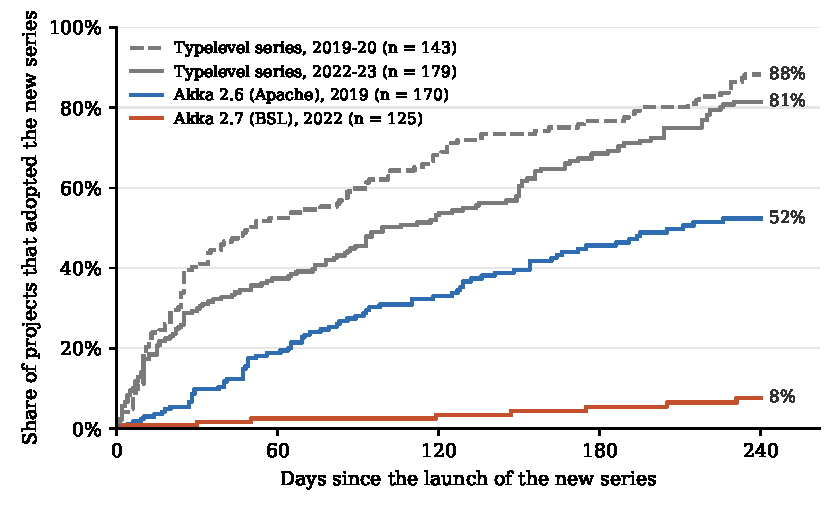
\includegraphics[width=0.78\textwidth]{fig_launch_uptake.pdf}
\caption{Share of projects that adopted the new series, by days since its launch. Kaplan-Meier estimates for projects with a release within 365 days: each project is followed only until its last release, so projects that stop releasing do not count as non-adopters after that date. Typelevel series: fs2 2.1 and cats-effect 2.1 (2019--20), cats-effect 3.4 and fs2 3.4 (2022--23).}
\label{fig:launch}
\end{figure}

\paragraph{Timing of adoption.} Figure~\ref{fig:launch} shows adoption over time among projects that released within a year. The 2.6 cohort adopted gradually, reaching about half by day 240. The 2.7 cohort barely moved.

\paragraph{Where the non-adopters went.} Between the 2.6 and 2.7 launches the share of projects that kept the previous series rose by 0.14 (weighted, 95\% CI 0.03 to 0.26) at 240 days and by 0.23 at 365 days, with similar unweighted estimates. The share with no release also rose, by 0.15 weighted (0.03 to 0.27), but only by 0.07 unweighted (not significant), and at 365 days by 0.11 weighted and 0.01 unweighted. Part of the 240-day gap is timing: projects in the 2.7 cohort released later in the year. Among projects that did release, the response was a freeze: of the 100 active projects that did not adopt 2.7, 97 declared 2.6 in at least one release during the window (one of them also declared Pekko), and the other three published only releases that declared no Akka. Extending the freeze claim to whole cohorts, including projects that stopped releasing, would require the rise in inactivity to be smaller than the rise in freezing and not significant. In the weighted estimate it was neither, so the paper makes the freeze claim only for projects that kept releasing, and reports that the license change may also have reduced activity.

\section{Panel evidence and the end of patches}\label{sec:panel}

The second design uses a panel with one row per project and calendar quarter. The outcome, M1, is the quarterly upgrade rate: among quarters in which a project published a release that still declares the supplier, the share in which a release raised the declared version. It counts patches within the open series as well as moves into restricted versions. The test is whether, after the event, M1 fell for Akka dependents relative to the comparison group, that is, whether the coefficient on $D=\text{Treated}\times\text{Post}$ is negative. The regression has project and quarter fixed effects, which remove each project's average level and the shocks common to a quarter. The comparison projects are weighted to resemble the treated ones (ATT propensity weights), and standard errors are clustered by owner. The panel runs from 2020Q4 to 2025Q3; the reference quarter is 2022Q2 and the event quarter, 2022Q3, is excluded.

\begin{table}[t]
\centering
\begin{threeparttable}
\caption{Panel estimate and robustness}\label{tab:panel}
\small
\begin{tabular}{lcc}
\toprule
Specification & Akka & Elasticsearch \\
\midrule
Primary: M1, project and quarter FE, ATT weights & $-0.297$ $[-0.41,-0.18]$ & $+0.032$ $[-0.06,0.13]$ \\
\quad wild cluster bootstrap $p$ / randomization inference $p$ & $<0.0001$ / $<0.0005$ & $0.52$ / $0.46$ \\
Balanced non-switchers & $-0.233$ $[-0.36,-0.11]$ & $+0.044$ $[-0.05,0.14]$ \\
Calendar-adjusted M1 & $-0.269$ $[-0.39,-0.15]$ & $+0.002$ $[-0.10,0.10]$ \\
Unweighted & $-0.300$ $[-0.39,-0.21]$ & $+0.016$ $[-0.07,0.10]$ \\
Against cats-effect only & $-0.300$ $[-0.42,-0.18]$ & \\
Excluding the top three owners per group & $-0.260$ $[-0.37,-0.15]$ & $+0.040$ $[-0.06,0.14]$ \\
\midrule
Event study: joint pre-period test $p$ & 0.078 & 0.0003 \\
Placebo break in the pre-period & $-0.157$ ($p=0.08$) & $+0.124$ ($p=0.004$) \\
Rambachan-Roth breakdown $\bar M$, average post effect & $\le 0.05$ & 0 \\
Linear extrapolation of the pre-trend ($\Delta^{SD}(0)$), 95\% set & $[-0.23,0.40]$ & $[-0.56,-0.11]$ \\
\bottomrule
\end{tabular}
\begin{tablenotes}\footnotesize
\item Akka: 385 treated and 545 comparison projects, 560 owner clusters, 4,307 project-quarters. Elasticsearch: 290 treated and 260 comparison projects. Brackets: 95\% confidence intervals with owner-clustered standard errors. Randomization inference compares the estimate with those obtained when treatment is reassigned at random across owners. Rambachan-Roth bounds computed with HonestDiD 0.2.8 on the event-study coefficients; the breakdown is the smallest $\bar M$ on a grid of step 0.05 at which the robust interval for the average post-period effect includes zero.
\end{tablenotes}
\end{threeparttable}
\end{table}

Table~\ref{tab:panel} reports the estimates. The primary estimate is $-0.297$ (SE 0.059), with $p<0.001$ under clustered standard errors, the wild cluster bootstrap and randomization inference, and the estimate stays between $-0.22$ and $-0.34$ across outcome codings, weights, fixed effects, comparison libraries, owner exclusions and windows. For Elasticsearch it stays near zero.

The estimate does not survive a sensitivity analysis for parallel trends. An event study estimates the gap between treated and comparison projects separately for each quarter, relative to the reference quarter. For Akka these gaps decline before the event, from 0.32 in 2020Q4 to zero in the reference quarter (joint test $p=0.078$). Part of this is the supplier's release calendar: Akka released four patches between October 2020 and February 2021 and none between 2.6.19 in March 2022 and 2.6.20 in September 2022. \citet{rambachan2023} show how to bound the estimate when the trends may diverge after the event by up to $\bar M$ times the largest quarter-to-quarter change seen before it. The confidence set for the average post-event effect includes zero already at $\bar M=0.05$, and extending the pre-event trend in a straight line removes the effect. Robustness to a divergence as large as the largest pre-event change would need a breakdown value of at least 1; here it is at most 0.05, so I report the panel estimate as fragile. The launch design was developed in response.

\begin{figure}[t]
\centering
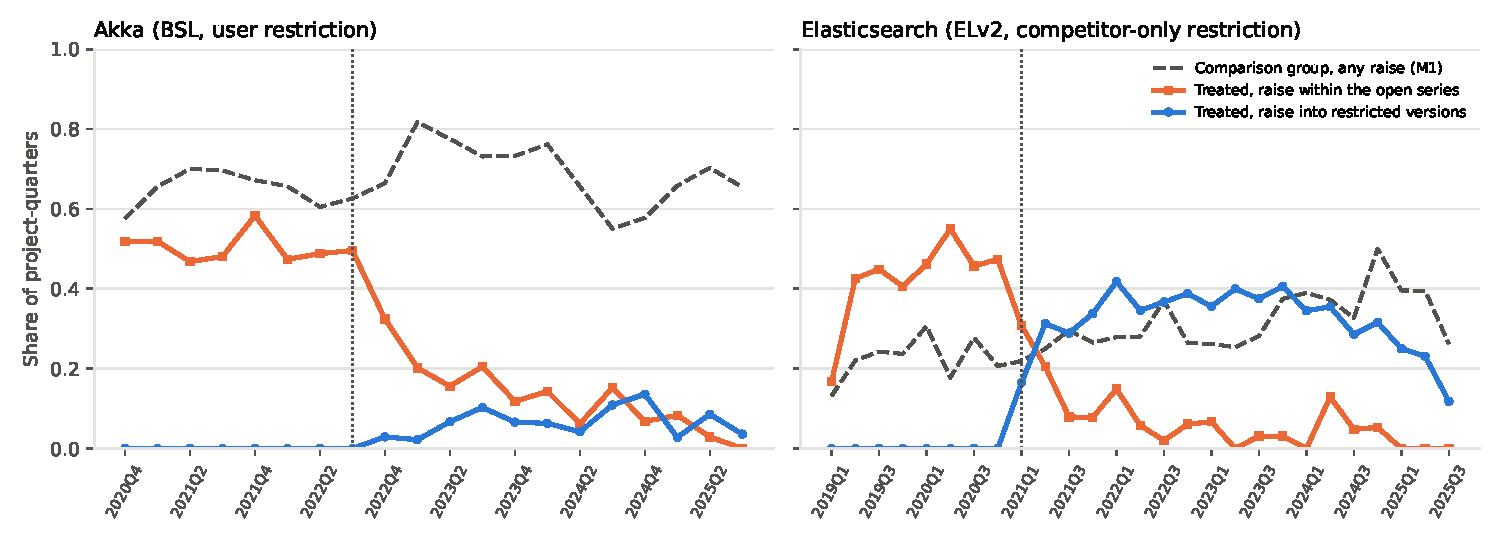
\includegraphics[width=\textwidth]{fig4_decomposition.pdf}
\caption{Where upgrades went. Share of treated project-quarters with a raise within the last open series and with a raise into restricted versions, and the comparison group's upgrade rate. Dotted lines mark the relicensing announcements.}
\label{fig:decomp}
\end{figure}

\paragraph{Decomposition.} Figure~\ref{fig:decomp} splits M1 into raises within the open series and raises into restricted versions (prediction P4); this split needs no comparison group. After both events no new open versions were released, so raises within the open series had to fall. In Elasticsearch, raises into restricted versions almost fully replaced them: they occurred in 35\% of project-quarters after the event, against 43\% for open-series raises before it. In Akka they did not: 6\%, against 50\%. The open-series raises that remain are mostly catch-up moves to 2.6.20 and 2.6.21. Restricted versions were available throughout, so the fall in Akka upgrading reflects projects declining them.

\paragraph{Status at the horizon.} At 30 September 2025, among all treated Akka projects including inactive ones, 22\% were frozen, 6\% had upgraded to restricted versions, 10\% had switched to Pekko, 7\% published both and 4\% had removed Akka; 51\% had released nothing since the event. Among projects that released, there were 0.26 upgraders per frozen project for Akka and 0.74 for Elasticsearch.

\paragraph{The end of patches and the fork.} Of 129 Akka projects frozen at 30 June 2023, 39 had moved to Pekko (16 switched, 23 published both) by 30 June 2024, 5 had upgraded to BSL versions and 2 had removed Akka (prediction P5). These shares are descriptive. Before Pekko's core release on 10 July 2023 switching and dual publishing were impossible (Section~\ref{sec:model}), so their rate before that date is zero whatever projects wanted. Comparing switching before and after the fork's arrival therefore measures how many projects switched once switching became possible. This would happen whatever the reason for freezing, so it cannot separate the channels.

A narrower question can be answered causally (prediction P6): once the fork's core existed, did a project switch more after the last port it needed arrived? Before that date switching was already possible, since a project could port a missing library itself, replace it or drop the feature, so a difference would reflect projects' choices. The data have little variation for this question. Of 206 active projects, 169 had every port they needed by the third quarter of 2023, when the fork's own modules arrived; 20 received their last port later, and 17 never did. The dates of third-party ports also responded to demand: popular libraries were ported sooner (Spearman rank correlation $\rho=-0.43$ between the number of dependents and the port date). With so little variation, and port dates that respond to demand, I treat the port-availability analysis as descriptive only. The one pattern it shows matches the direction of this channel: frozen projects still missing a port in September 2023 took BSL versions more often (3 of 24, against 2 of 105 for projects with every port; Fisher's exact test $p=0.044$). Most projects in both groups stayed frozen.

\section{Why did dependents freeze?}\label{sec:channels}

\subsection{Restriction scope: Akka against Elasticsearch}

Prediction P3 attributes the difference between the two events to the legal cost. Two contrasts that do not rely on the panel outcome M1 fit this reading. First, among projects that ever declared a restricted version after the event, 9 of 44 Akka projects later moved to the fork, against 1 of 65 Elasticsearch projects (Fisher's exact test, $p=0.001$). An Akka project moving from BSL versions to Pekko gives up the improvements released after 2.6, a loss that in the model only the legal cost or hold-up can justify. Elasticsearch projects that left restricted versions went most often to Elastic's own Apache client (8 of 16). Second, in their issue trackers Akka dependents give the license as their reason far more often, while Elasticsearch dependents mostly give technical compatibility (Section~\ref{sec:said}): because Elastic's clients refused to connect to other servers from version 7.14, a library chose the client that worked with the server its users ran.

The contrast is between two events, and they differ in more than restriction scope. OpenSearch had a large sponsor from the start, Elastic had a public conflict with AWS before 2021, and Elastic offered an Apache client path that Lightbend did not. The direction in which each of these affects the comparison is unknown. The difference between the two events in the panel estimate ($-0.33$) carries over the pre-trend problems of both panels and is not robust, so the comparison between the events is descriptive.

\subsection{What dependents said}\label{sec:said}

I searched the issues and pull requests of 631 treated repositories through the documented GitHub search API, with a fixed set of queries. After removing items written by automated update tools (Scala Steward, Dependabot, Snyk), 1,096 items in 135 repositories mention the fork or the supplier's license. Each repository was coded from up to four items selected by a fixed rule, against a codebook, a list of codes with their definitions. A language model assigned the codes for all repositories.\footnote{The model was Claude Opus 5.5 (\texttt{claude-opus-5-5}), used interactively, reading the selected items in batches with the codebook as its instruction. Sampling settings were not controlled, so the codes cannot be regenerated exactly; the inputs, codebook and codes are in the replication package. A simple keyword rule agrees with the model on which repositories are relevant ($\kappa=0.76$) but not on motives ($\kappa\le0.38$). Motives therefore cannot be coded by keywords alone; this comparison does not test whether the model's motive codes are right.}

\paragraph{Human validation.} The author coded a sample of 60 repositories without seeing the model's codes, using a page that showed the same items. The sample was drawn first from repositories the model had coded as citing the license or trust, and the rest at random. The model codes are accepted if Cohen's $\kappa$ is at least 0.60 for both ``license given as a reason'' and ``technical compatibility''. Agreement was 0.90 (95\% CI 0.77 to 1.00) and 0.80 (0.58 to 0.95), so the model codes are used. Agreement on which repositories were relevant was lower ($\kappa=0.35$). In all nine disagreements the item was a routine version update inside the fork, which the human coded as not relevant and the model as relevant. This enlarges the model's set of relevant repositories, so its shares of repositories citing each motive are, if anything, understated. Before coding, the author had seen the overall shares from the model's codes, but not the code of any single repository. There was no second human coder.

\paragraph{Motives.} Where a motive is stated (40 Akka and 14 Elasticsearch repositories), the license is the reason in 95\% of Akka cases and 43\% of Elasticsearch cases, and technical compatibility is the reason in 93\% of Elasticsearch cases. On the validation sample the human codes give the same contrast: the license is a reason in 81\% of relevant Akka repositories and 23\% of Elasticsearch ones; technical compatibility in 12\% and 50\%. When a project explains how the license affects it, the reason is more often a license-compatibility rule than a fee: a project under the Eclipse Public License cannot include BSL code; a project cannot keep its own open license while depending on BSL code; the automated license checks in a project's build pipeline fail; downstream users would inherit the BSL. On the Elasticsearch side the legal cases are Apache Software Foundation projects. The foundation allows a dependency only if its license meets the Open Source Definition, the standard kept by the Open Source Initiative, whatever the license's scope; it lists the SSPL among the licenses its projects may not use. Whether a project is exposed therefore depends on its own governance rules as well as on whom the license restricts. Language about trust or fear of future restrictions is rare: two of 48 relevant repositories in the human-coded sample, one in each event, and the human and the model found it in different repositories.

\subsection{A within-event test of exposure}

If the legal cost works through a library's users, libraries with more downstream users should have been more reluctant to take BSL versions. I measure each project's exposure as the number of distinct packages outside its own repository that listed one of its packages as a direct, non-test dependency in releases published in the year before the launch, from deps.dev. The test asks whether the fall in adoption at the 2.7 launch was larger for projects with more downstream packages, using an interaction between this measure and the 2.7 cohort in the launch design. The legal channel predicts less adoption and more freezing. The interaction is close to zero: $+0.02$ for adoption ($[-0.05,0.09]$, $p=0.64$) and $-0.03$ for freezing ($p=0.56$). For Elasticsearch, where the model predicts no such difference, it is $-0.06$ ($[-0.14,0.01]$). The test has little power. Three quarters of projects have no observed downstream package, and the measure counts only open-source packages on Maven Central, the users least likely to be charged by the BSL. The test is therefore uninformative about the legal channel.

\subsection{Tests of the hold-up channel}

\paragraph{Spillover to the supplier's other libraries.} If hold-up moved Akka dependents, they should also have reduced their use of Lightbend's libraries whose license did not change: config, ssl-config, scala-logging and Slick, for configuration, secure connections, logging and database access. Among Akka dependents that used these libraries in the year before the event and released afterward, 43 of 46 still declared them two years later (excluding projects that removed Akka altogether). In the same comparison two years earlier, when no license changed, 49 of 52 did. Projects that switched to Pekko kept them (17 of 18). The test is large enough to detect a fall of about 15 points in the share that kept these libraries.

\paragraph{License keys.} The license keys required for new versions from October 2024 raised the cost of compliance for projects already on BSL versions but revealed nothing new about the supplier's willingness to change terms. If the cost of compliance drives decisions, projects on BSL versions should have left after this change. Of 23 projects on BSL versions in September 2024, 18 were still on them a year later, against 17 of 23 in the year before. The keys apply only to new versions, so projects could stay on older BSL versions without one, and the test has little power.

\paragraph{The change date.} Version 2.7.0 reverted to Apache 2.0 on 19 October 2025, three years after its release. If the legal cost alone had kept projects on 2.6, those still releasing should then have moved to 2.7, now under Apache 2.0. Of 21 projects still releasing Akka-only builds after the conversion, one did. I designed this test after seeing the conversion mentioned in the projects' discussions. The result weakens the view that the legal cost alone explains the long-run freeze. But by 2025 the projects still releasing were few and mostly in maintenance mode, a three-year-old version offered them little, and hold-up, inattention or a fixed policy of not using Akka beyond 2.6 would explain the result equally well.

\paragraph{Summary.} Three pieces of evidence point to the legal cost, and in particular to rules on license compatibility that pass from a library to the projects that depend on it. Elasticsearch dependents, who faced no legal cost, kept upgrading. Akka dependents named license conflicts as their reason, in statements whose coding a human check confirmed. And Akka dependents kept using Lightbend's other libraries, which is hard to reconcile with distrust of the company. None of the evidence supports hold-up directly. But the test based on downstream users is uninformative, and no single test cleanly separates the channels, so the legal explanation remains suggestive.

\section{Threats to validity}\label{sec:threats}

\paragraph{Order of the analyses.} The launch design was chosen when the 2.7 result was already partly known (Section~\ref{sec:launch}), so it may fit that result better than a design chosen beforehand would. The earlier cohorts, the benchmarks and the robustness checks were computed afterward, and the outputs of every estimate are in the replication package.

\paragraph{Composition of the cohorts.} The projects in the 2.7 cohort were older and larger than those in earlier cohorts. Reweighting handles this for the 2.6 cohort but not for the 2015 and 2017 cohorts (Section~\ref{sec:launch}), and two results do not depend on composition: the comparison of the same projects across launches and the Lee bounds.

\paragraph{Benchmarks.} Section~\ref{sec:launch} notes the limits of the two benchmarks. One more applies to both. Automated update tools such as Scala Steward spread between 2019 and 2022; they raise adoption in all groups and would bias the comparison only if their spread differed by group.

\paragraph{Activity and inactivity.} Besides projects that moved their publishing off Maven Central (Section~\ref{sec:data}), a project that moved to new artifacts declaring neither Akka nor Pekko would appear inactive. Both cases would make adoption or leaving look lower, and inactivity higher, than they were. To bound this error, I listed the version tags in the GitHub repository of every Akka project coded as frozen or as publishing no release (289 projects, of which 264 repositories could be reached). In 31 of the 183 reachable projects with no release, and in 19 of the 81 frozen ones, the highest version tag is above the highest version of the project's Akka-dependent artifacts on Maven Central. This is an upper bound on misclassification: tags carry no dates, and a later tag can also mark a version released before the event but never published, a release of other artifacts without Akka, or a package published under a new name. Even if every flagged project had in fact kept releasing, at least 152 of the 183 reachable projects coded as publishing no release show no sign of a later version.

\paragraph{Declared versus used.} A POM records what a project declared. Applications that use the project can override these versions, and shaded code does not appear. The validation against repository build files compares the coding with each project's build configuration; it cannot show which versions run in production.

\paragraph{Channel evidence.} Besides the limits noted in Section~\ref{sec:channels}, the statements come only from projects that chose to discuss their decision, about a quarter of the Akka risk set.

\section{Discussion}\label{sec:discussion}

\paragraph{What is identified.} The launch design identifies the effect of the BSL, together with the release pattern that came with it, on adoption of the new series by open-source projects that were on the previous series. It measures this effect against Akka's own earlier launches and against libraries without a license change. It does not identify the effect on all Akka users or on applications that do not publish to Maven Central. The panel estimate, which would have measured the effect on the upgrade rate over three years, does not survive plausible departures from parallel trends.

\paragraph{Who is observed.} The companies the BSL charges, which build closed applications, are not observed. For them the license is a direct cost, scaled by the cores they run. The libraries observed here pay nothing, yet they froze, which suggests that the legal cost is passed along the chain of dependencies, from the companies that would pay to the libraries they use. A commercial user facing a per-core bill can also run Akka on fewer cores, a response that registry data cannot show.

\paragraph{Implications.} For a supplier, a license that restricts end users can also stop the library's own ecosystem from moving with it, and push that ecosystem toward the fork once the open version loses support. A license that restricts only competitors, as Elastic's did, kept dependents on the supplier's versions. The fork also limits what the supplier can charge: once the fork and the ports a project needs exist, leaving costs the project little. For the ecosystem, part of the cost of a relicensing is outdated dependencies: three years after the event, more treated Akka projects were frozen on a version without security fixes (22\%) than had moved to the fork (17\%, counting dual publishers) or to the restricted versions (6\%). For foundations and policy makers, license rules travel along the chain of dependencies, so a restriction aimed at one kind of user also binds many projects it was not aimed at.

\section*{Data and code availability}
The data and code needed to reproduce every result in this paper are available at \url{https://github.com/TJ-overflow/relicensing-dependents} and archived on Zenodo at \url{https://doi.org/10.5281/zenodo.24440614}. The coded dataset of dependents' choices is released under CC BY 4.0 and the code under the MIT license. Issue and pull-request text and GitHub profile fields are not redistributed; the package includes the scripts that re-collect them from public sources.

\section*{Use of AI tools}
The author used Claude (Anthropic), an AI assistant, to help write the data-collection and analysis code and to edit the text, in addition to the coding of motives described in Section~\ref{sec:said}. The author directed the research, reviewed the code and results, and takes full responsibility for the content.

\bibliographystyle{plainnat}
\bibliography{references}

\end{document}
